% vim: set tw=78 sts=2 sw=2 ts=8 aw et ai:

In order to conduct our tests, we employ an updated version of the framework
we have previously used to analyze MPTCP on its own\cite{sem1}. The current
testbed features two hosts with a single Ethernet link between them. The
Ethernet link serves as a carrier for two OpenVPN tunnels, one over UDP and
the other over TCP. This setup allows us to impose rate-limiting on the Ethernet
interface, which will then propagate on the tunnel interfaces. At the same
time, we can run MPTCP over the OpenVPN tunnels and observe how traffic is
moved to less congested paths and aggregated. For the most part, we have
eliminated encryption and message authentication since that induces
computational overhead in an already burdened environment. A difference from
our previous testbed is that we use netperf to measure the throughput since it
has proven to be more stable, while yielding similar results.

We cannot properly establish the benefits of MPTCP without measuring the
achievable throughput using a single tunnel. Figures \ref{fig:udp} and
\ref{fig:tcp} show the results for a UDP tunnel and a TCP tunnel,
respectively.

\begin{figure}
  \centering
  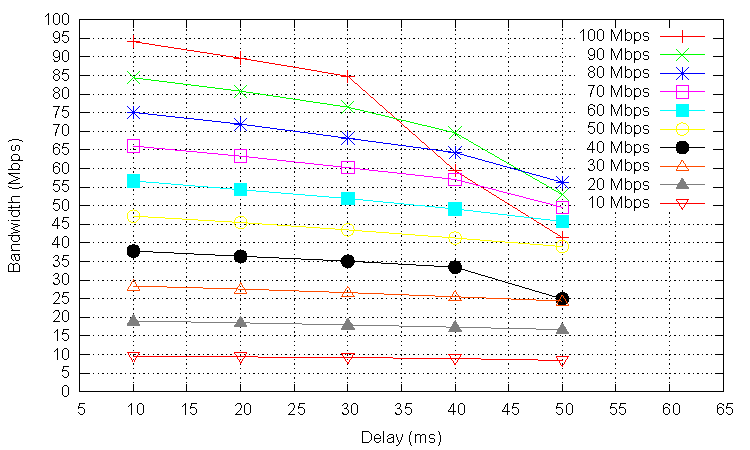
\includegraphics[width=\textwidth]{img/test-udp}
  \caption{UDP tunnel throughput}
  \label{fig:udp}
\end{figure}

\begin{figure}
  \centering
  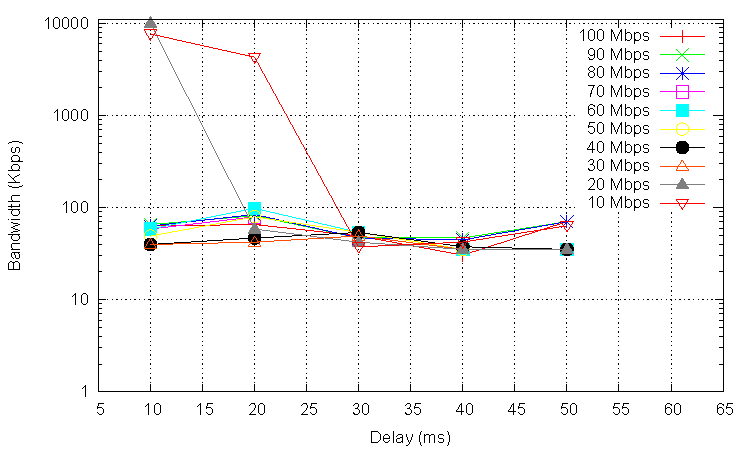
\includegraphics[width=\textwidth]{img/test-tcp}
  \caption{TCP tunnel throughput}
  \label{fig:tcp}
\end{figure}

In the case of the UDP tunnel, we notice that for lower link capacities, the
UDP tunnel manages to offer throughput close to the maximum achievable values.
That does not apply for larger bandwidths and delay. We consider that the root
cause for this is the overhead introduced by copying the data from the tunnel
device in users-pace, in the OpenVPN process, and then back to kernel-space to
be sent via the Ethernet device.

The TCP tunnel exhibits poor results. Most throughput values are in the range
of 30 - 70 Kbps, with a few exceptional cases where we reach throughput up to
10 Mbps. This undeterministic and unsatisfactory result can be explained by
taking into account the nature of our testbed. Not only are we copying large
amounts of data between user-space and kernel-space, in a virtualized
environment, but we are also attempting to run TCP traffic over a TCP tunnel.
By default, the Linux kernel uses the CUBIC congestion control algorithm with
regards to TCP connections. While this implementation has proven to be
efficient, the fact that we are encapsulating TCP traffic in TCP means that
the two instances of CUBIC will conflict each other. We believe these are the
factors that lead to such poor performance.

Having set the baseline for what can be done using a single tunnel, we have
also conducted tests using two tunnels, using MPTCP. We have configured MPTCP
to make use of the Olia congestion control algorithm with the goal of
observing how traffic is shifted to less congested paths, in our case the UDP
tunnel, despite the initial connection being made over the congested path, in
our case the TCP tunnel. A relevant factor in assisting MPTCP was configuring
the buffer size for a connection. We have based our tests in this regard while
taking into account the bandwidth-delay product of the link.

\begin{figure}
  \centering
  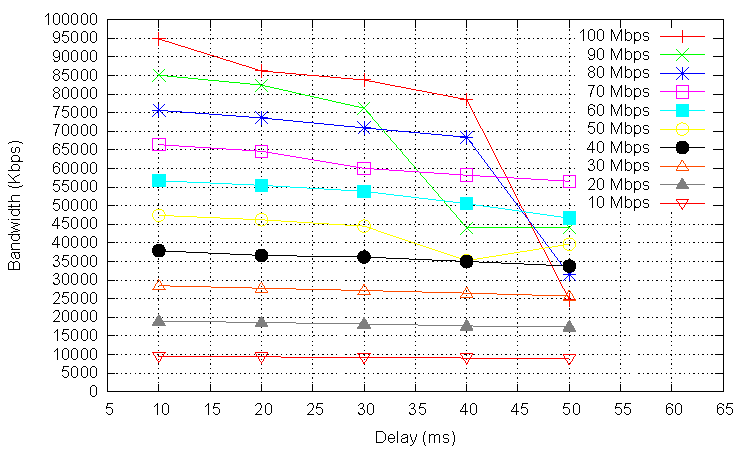
\includegraphics[width=\textwidth]{img/test-mptcp-05}
  \caption{UDP and TCP tunnels throughput, $buffer size = 0.5 \times BDP$}
  \label{fig:mptcp-0.5}
\end{figure}

\begin{figure}
  \centering
  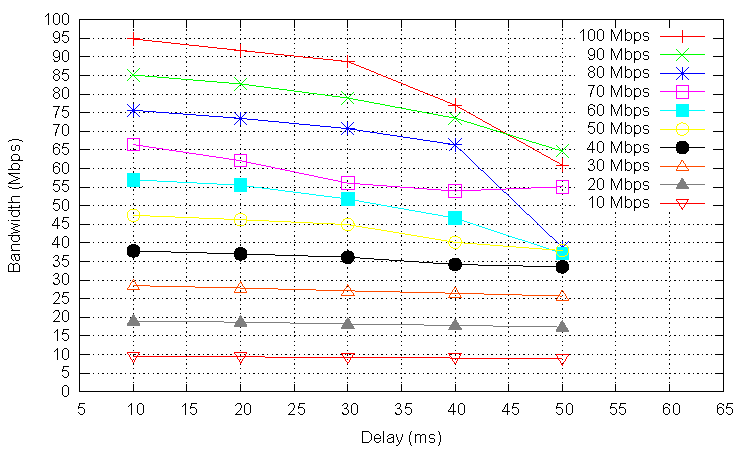
\includegraphics[width=\textwidth]{img/test-mptcp}
  \caption{UDP and TCP tunnels throughput, $buffer size = BDP$}
  \label{fig:mptcp}
\end{figure}

Figures \ref{fig:mptcp-0.5} and \ref{fig:mptcp} show the throughput when the
buffer size was either half or equal to the bandwidth-delay product. In most
cases, the results are similar or better when compared to single UDP and
single TCP. However, towards the end of the spectrum, that is for high
bandwidths and high delays, the throughput is less than that of a single UDP
tunnel, with the problem being more obvious when the buffer size is half of
the BDP. The cause lies in the fact that the buffer is insufficient and cannot
hold all the necessary packets.

\begin{figure}
  \centering
  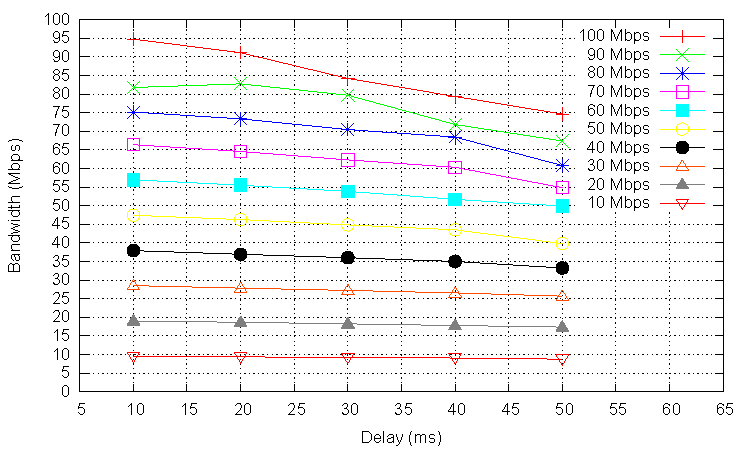
\includegraphics[width=\textwidth]{img/test-mptcp-2}
  \caption{UDP and TCP tunnels throughput, $buffer size = 2 \times BDP$}
  \label{fig:mptcp-2}
\end{figure}

Figure \ref{fig:mptcp-2} presents the throughput when the buffer size is twice
the BDP. Using this configuration, we notice that even at the high end of the
test spectrum, the results are better than single UDP or single TCP, as well
as the two previous tests. We still are not able to fully make use of the link
capacity, but we attribute this drawback to reasons mentioned above, namely
virtualization and copying of data.

While attempting to maximize link usage, we have also tested with buffer sizes
which are three times and four times the bandwidth-delay product. Figures
\ref{fig:mptcp-3} and \ref{fig:mptcp-4} summarize our results. While the lower
spectrum is comparable to previous tests, beyond an available capacity of 60Mbps
and a delay of 30ms we notice a drop in throughput, with an even greater drop
in performance in the case of four times the BDP. This is a consequence of
granting too much memory for network buffers.

\begin{figure}
  \centering
  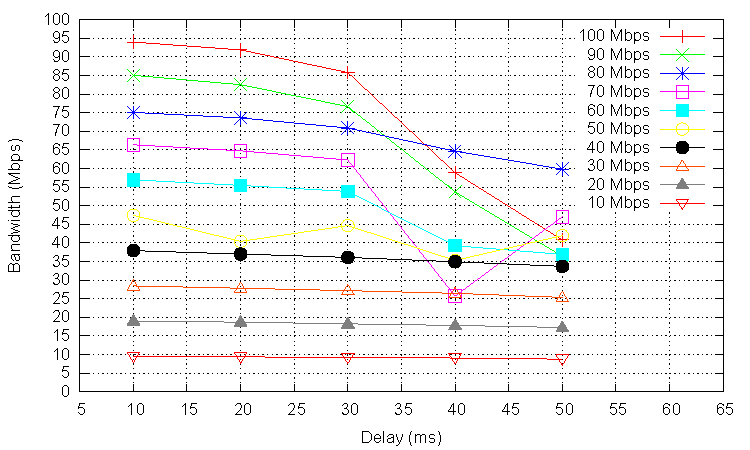
\includegraphics[width=\textwidth]{img/test-mptcp-3}
  \caption{UDP and TCP tunnels throughput, $buffer size = 3 \times BDP$}
  \label{fig:mptcp-3}
\end{figure}

\begin{figure}
  \centering
  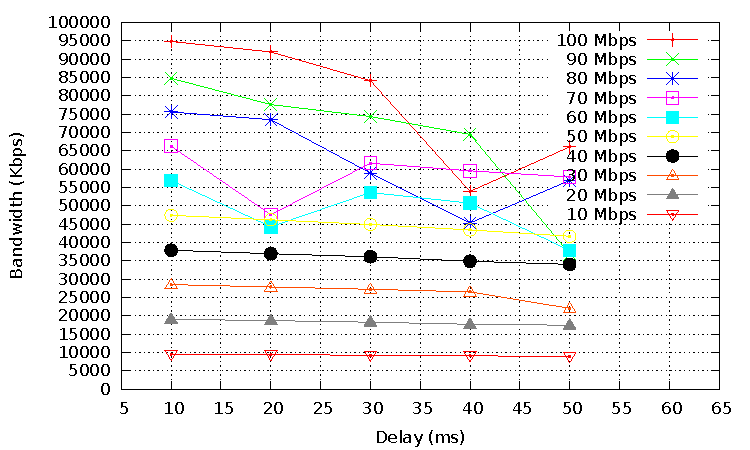
\includegraphics[width=\textwidth]{img/test-mptcp-4}
  \caption{UDP and TCP tunnels throughput, $buffer size = 4 \times BDP$}
  \label{fig:mptcp-4}
\end{figure}

\begin{figure}
  \centering
  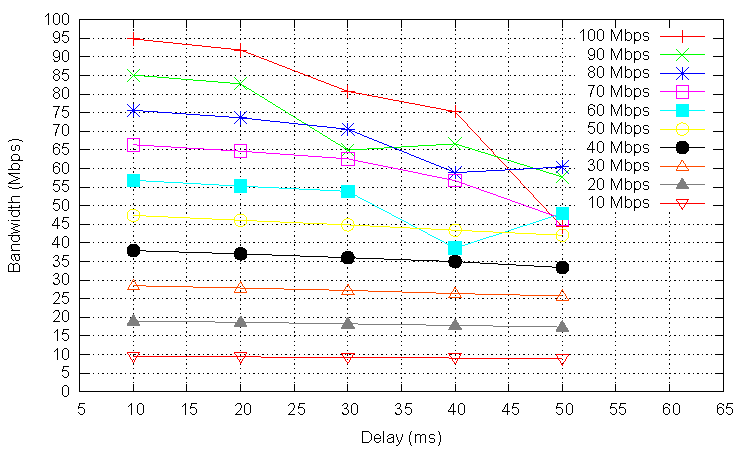
\includegraphics[width=\textwidth]{img/test-mptcp-2-crypto}
  \caption{UDP and TCP tunnels throughput, $buffer size = 2 \times BDP$, Blowfish CBC and SHA1}
  \label{fig:mptcp-2-crypto}
\end{figure}

Since our tests indicate that a buffer size twice the bandwidth-delay product
yields the best results, we have also looked at how OpenVPN's normal mode of
operation influences throughput. By default, OpenVPN uses Blowfish in CBC mode
to encrypt the information and SHA1 as a message authentication code. The
results are outlined in \ref{fig:mptcp-2-crypto}. Some irregularities can be
noticed, but we attribute those to the fact that this test incurs additional
overhead due to the increased computation inherent to encryption.

